\documentclass[10pt]{beamer}

% packages de base
\usepackage[frenchb]{babel}
\usepackage[utf8]{inputenc}
\usepackage[T1]{fontenc}

% package pour les images
\usepackage{graphicx}

% package pour les algorithmes
\usepackage[french,lined]{algorithm2e}

% package pour le code
\usepackage{minted}

% package pour les schémas 
\usepackage{tikz}
\usetikzlibrary{shapes,snakes,calc}

% package pour les vidéos
\usepackage{multimedia}
%\usepackage{media9}

%----------------------------------------------------------------------

% couleurs et style
\usecolortheme[RGB={25,110,170}]{structure}
\usetheme{Madrid} 
\setbeamersize{text margin left=1cm, text margin right=1cm} 
\useoutertheme{umbcfootline} 
\setfootline{\insertauthor \hfill \insertshorttitle \hfill \insertframenumber/\inserttotalframenumber} 

% profondeur du sommaire
\setcounter{tocdepth}{1}

% rappelle le sommaire à chaque nouvelle section
\AtBeginSection[] {
  \begin{frame}{\large Sommaire}
    \tableofcontents[currentsection]
    \addtocounter{framenumber}{-1}
  \end{frame}
} 

% titre, auteur...
\title[titre court] {titre long}
\author{auteur}
\institute{LISIC, ULCO}
\date{7 juin 2016}

%----------------------------------------------------------------------

\begin{document}

% slide de titre
\begin{frame}
  \maketitle
\end{frame}

% sommaire
\begin{frame}{\large Sommaire}
  \tableofcontents
\end{frame}

%----------------------------------------------------------------------

\section{Les images de synthèse,}

% une image
\begin{frame}{\large \insertsection}
  \begin{block}{Photographie}
      \begin{center}
          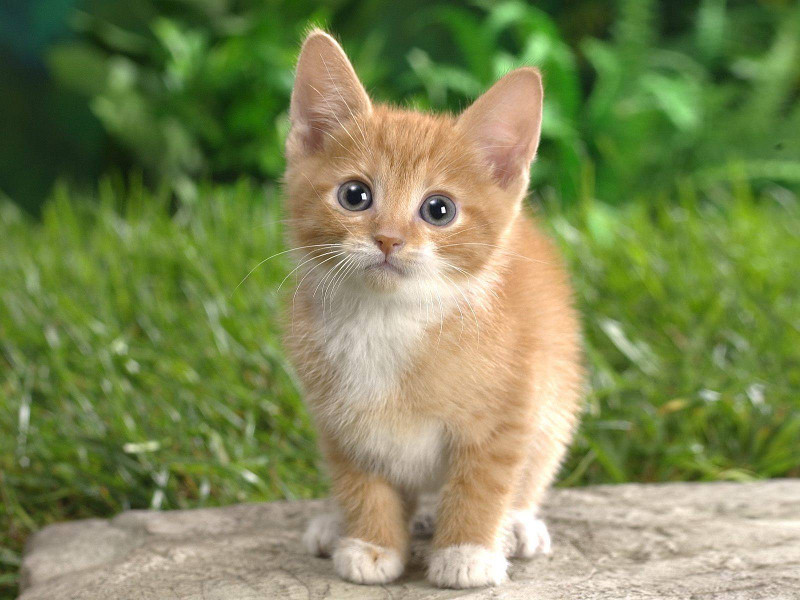
\includegraphics[width=6cm]{images/chaton.jpg}
          \\ http://www.findcatnames.com
      \end{center}
  \end{block} 
\end{frame}

% des images sur deux colonnes, dans un tableau
\begin{frame}{\large \insertsection}
    \begin{block}{Images de synthèse non-photoréalistes}
        \begin{center}
            \begin{tabular}{c c}
                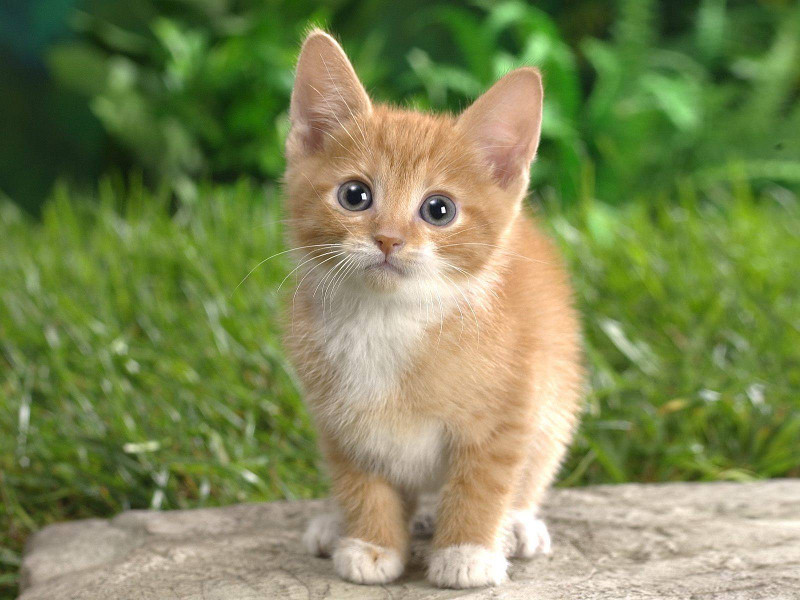
\includegraphics[height=2cm]{images/chaton.jpg}
                &
                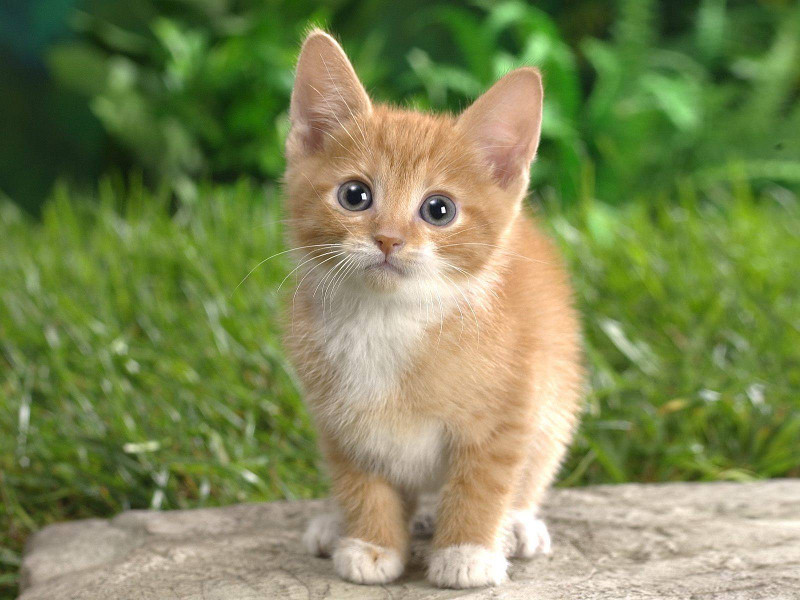
\includegraphics[height=2cm]{images/chaton.jpg}
                \\ 
                ATI Demo, 
                &
                TU Delft Graphics, 
                \\
                Non Photorealistic Rendering
                &
                Exposure Render 
            \end{tabular}
        \end{center}
    \end{block} 
\end{frame}

% une vidéo 
% attention, seuls certains viewers PDF supportent les vidéos (par ex. okular)
\begin{frame}{\large \insertsection}
    \begin{block}{Travaux au LISIC : perception du bruit}
        \centering
        \pgfdeclareimage[width=7cm]{giphy}{images/giphy.png}
        \movie[loop,autostart]{\pgfuseimage{giphy}}{images/giphy.mp4}
    \end{block} 
\end{frame}

%----------------------------------------------------------------------

\section{un problème de radiométrie}

% liste d'items et image sur deux colonne, dans des minipages
\begin{frame}{\large \insertsection}
    \begin{block}{Transport de la lumière }
        \begin{minipage}{0.45\textwidth}
            \begin{itemize}
                \item Soit une scène virtuelle, composée :
                    \begin{itemize}
                        \item d'émetteurs,
                        \item de réflecteurs et
                        \item de récepteurs de lumière.
                    \end{itemize}
                \item On veut calculer la \\ « lumière reçue ».
                \item [$\rightarrow$] Grandeur physique à mesurer ?
                \item [$\rightarrow$] Propriétés du transport de la lumière ?
            \end{itemize}
        \end{minipage}
        ~~
        \begin{minipage}{0.5\textwidth}
            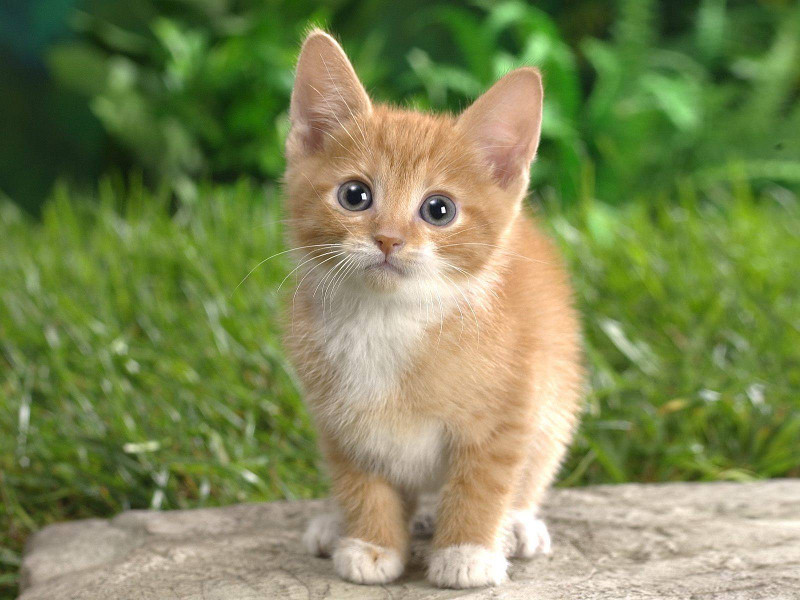
\includegraphics[height=3cm]{images/chaton.jpg}
        \end{minipage}
    \end{block} 
\end{frame}

% liste d'items puis images
\begin{frame}{\large \insertsection}
    \begin{block}{Flux}
        \begin{itemize}
            \item puissance totale 
            \item notation : $\Phi \quad [W]$
            \item souvent utilisé pour décrire une source \\
                (ne pas confondre avec la consommation électrique)
        \end{itemize}
        \begin{center}
            \begin{tabular}{c c c}
                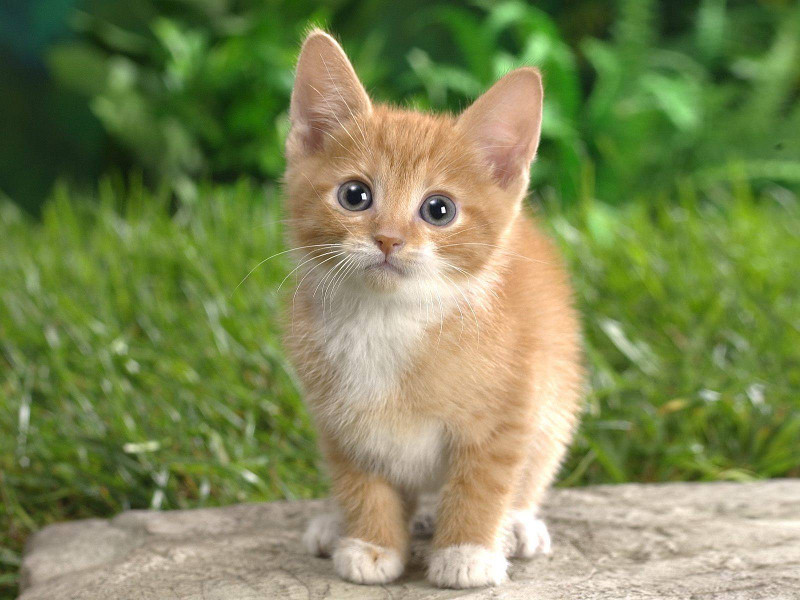
\includegraphics[width=2cm]{images/chaton.jpg} &
                ~~~~~~ &
                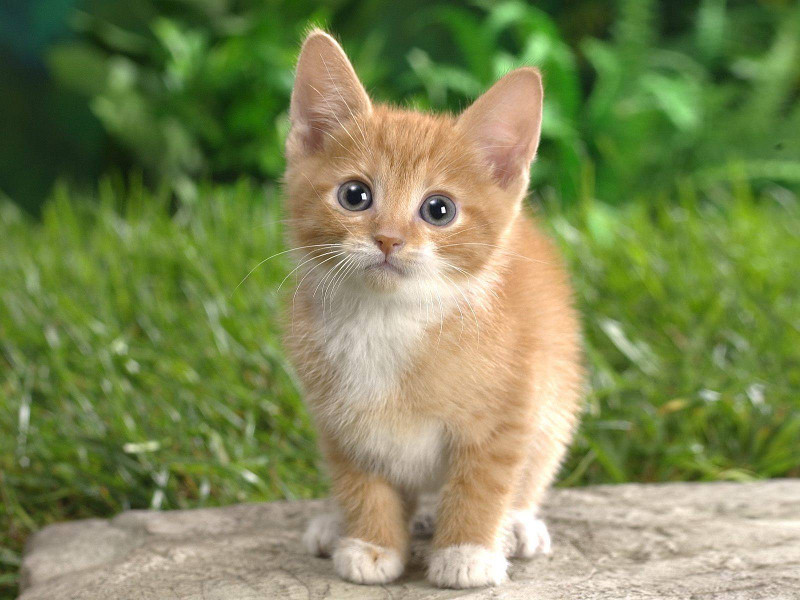
\includegraphics[width=2.5cm]{images/chaton.jpg} \\
                flux reçu & & flux émis 
            \end{tabular}
        \end{center}
    \end{block} 
\end{frame}

% formules de math
\begin{frame}{\large \insertsection}
    \begin{block}{Formulation « trois points » }
        \begin{itemize}
            \item $L_i(x', \omega_i') = L_o(x, \omega_o) = L(x \rightarrow x')$ 
            \item changement de variable :
                \scriptsize
                $$\sigma_{x'}^\perp(\omega_i') = G(x \leftrightarrow x') A(x) \text{ où } G(x \leftrightarrow x') = V(x \leftrightarrow x') \frac{|\cos \theta_o \cos \theta_i'|}{|| x - x' ||^2}$$
                \normalsize
        \end{itemize}
    \end{block} 
\end{frame}

%----------------------------------------------------------------------

\section{traité par des algorithmes probabilistes.}

% algorithme
\begin{frame}{\large \insertsection}
    \begin{block}{Metropolis Light Transport \cite{Veach1997}}
        \begin{algorithm}[H]
            \DontPrintSemicolon
            \PourCh{pixel de l'image}{
            $\bar x_0 \leftarrow$ choisir un chemin initial \;
            \Pour{$i$ de 1 à $N$}{
                $\bar y \leftarrow$ mutation$(\bar x_{i-1})$ \;
            $\bar x_i \leftarrow \left\{ \begin{array}{l} \bar y \text{ avec la probabilité } a(\bar y | \bar x_{i-1}) \\ \bar x_{i-1} \text{ sinon } \end{array} \right.$ \;
            ajouter la contribution de $\bar x_i$ au pixel \;
            }
            }
        \end{algorithm}
    \end{block} 
\end{frame}

% code source
\begin{frame}[fragile]{\large \insertsection}
    \begin{block}{Fichier principal}
        \begin{minted}[fontsize=\footnotesize]{c++}

  #include <Herve/Herve.hpp>
  #include <HerveOvr/HerveOvr.hpp>
  Herve::DisplayDevice * gPtrDisplayDevice; // périphérique d'affichage
  Scene gScene; // scène implémentant le monde virtuel voulu
  // ...
  int main() {
      // ...
      gPtrDisplayDevice->initDevice();
      gPtrDisplayDevice->initDisplay( /* ... */ );
      gScene.init( /* ... */ ); 
      bool executionEnCours = true;
      while (executionEnCours) {
          // ...
          gPtrDisplayDevice->render(&gScene);
      }
      return 0;
  }

        \end{minted}
    \end{block} 
\end{frame}

% schémas tikz
\begin{frame}{\large \insertsection}
    \begin{itemize}
        \item un schéma simple :

            \begin{center}
        \begin{tikzpicture}[thick,font=\scriptsize,scale=0.7]
            \node [orange] (S0) at (2, 0) {S0};%
            \node [blue] (S1) at (4, 0) {S1};%
            \node [red] (S2) at (2, 2) {S2};%
            \node [teal] (S3) at (4, 2) {S3};%
            \draw (S0) to (S1) to (S3) to (S2) to (S0);
            \draw (S1) to (S2);
            \draw[->] (0, 0) to (0, 1) node [above]{$y$};
            \draw[->] (0, 0) to (1, 0) node [right]{$x$};
            \draw[->,thick] (0, 0) to (-0.6, -0.6) node [right]{$~z$};
            \node () at (2.7, 0.5) {T0};%
            \node () at (3.3, 1.5) {T1};%
        \end{tikzpicture}%
            \end{center}

        \item un schéma plus compliqué :

            \begin{center}
        \begin{tikzpicture}[thick,font=\scriptsize]
            \foreach \i [count=\n] in {2,0,0,  4,0,0,  2,2,0,   4,2,0} {
                \node[draw,minimum height=4mm,minimum width=4mm, xshift=\n*4mm, yshift=-5mm](P\n){\i} ;
            }
            \foreach \c/\i [count=\n] in {orange/S0, blue/S1, red/S2, teal/S3} {
                \pgfmathtruncatemacro{\b}{\n*3}
                \pgfmathtruncatemacro{\a}{\b - 2}
                \draw [\c, decoration={ brace, mirror, raise=3mm ,amplitude=2mm}, decorate ] 
                (P\a.west) -- (P\b.east) node [pos=0.5,anchor=north,yshift=-5mm] (\i) {\i}; 
            }
            \foreach \c/\i [count=\n] in {orange/0, blue/1,  red/2, blue/1, teal/3,  red/2} {
                \node[draw,minimum height=4mm,minimum width=4mm, xshift=\n*4mm+1cm, yshift=-25mm](I\n){\i} ;
                \draw [->,\c ] (I\n) to[out=90,in=-90] (S\i); 
            }
            \foreach \c/\i [count=\n] in {T0, T1} {
                \pgfmathtruncatemacro{\b}{\n*3}
                \pgfmathtruncatemacro{\a}{\b - 2}
                \draw [decoration={ brace, mirror, raise=3mm ,amplitude=2mm}, decorate ] 
                (I\a.west) -- (I\b.east) node [pos=0.5,anchor=north,yshift=-5mm] {\i}; 
            }
            \node () at (-0.7, -0.5) {positions 3D} ;
            \node () at (0.5, -2.5) {indices} ;
        \end{tikzpicture}
            \end{center}

\end{itemize}
\end{frame}


% bibliographie
\nocite{*}
\begin{frame}{\large \insertsection}
  \begin{block}{Quelques références}
      \small
      \bibliographystyle{alpha}
      \bibliography{slides}
  \end{block} 
\end{frame}

% slide de fin
\begin{frame}
    \begin{center}
        Merci de votre attention !
    \end{center}
    \begin{center}
        Questions \& remarques ?
    \end{center}
\end{frame}

%----------------------------------------------------------------------

\end{document}

